\section{Tracing}
\label{sec:tracing}
Our aim in this work was to characterize the network interaction 
between Hadoop and its related network infrastructure and the impact this 
interaction has on applications. In addition to this we aimed to 
characterize the impact of Hadoop on a datacenter network, and the 
influence of the network - its topology, protocols, and scheduling - has on the 
end-to-end application behavior. We believe this work is a good first step 
towards a better understanding of the complexity of DISC framework's interaction
with the network. In this section we discuss the components of our initial tracing
infrastructure, Section~\ref{ssec:app} discusses application-level tracing, 
Section~\ref{ssec:low} discusses low-level tracing and lastly, 
Section~\ref{ssec:results} discussing some initial results that use our high/low-level
tracing mechanisms.

\subsection{Application-level Tracing}
\label{ssec:app}
Through the use of X-Trace~\cite{xtrace} we are able to expose causally related 
application-level events of a Hadoop job's execution. Each event that X-Trace
exposes provides us additional context about what other events came before it and
caused it to occur and similarly what events came after it. By creating X-Trace 
events for each TCP socket connect call we are able to discover the event history
for every TCP socket that is created throughout the lifetime of a job's execution.

We have augmented an X-Trace instrumented alpha version of Hadoop 2.0.4 to create 
X-Trace events for every TCP socket created. This enables us to gain a deeper insight
into every TCP socket by providing a history of events that triggered the socket and
the 5-tuple related to it (i.e. source IP/port, destination IP/port, and protocol).
Figure~\ref{fig:xtrace} is an example graphic that shows causally related events that
led to a TCP socket being created. Each event box contains a unique 16 character 
identifier and a short description of the event. The black box to the left of the 
figure represents additional information related to the event it points to. This includes 
a subset of information available for each event, such as if the event relates to a socket
connect call it displays the source IP/port and destination IP/port. Not displayed for space
reasons in the black text box is the stacktrace of function calls that led to this event. In 
addition to the event context information an event graph is produced for each job that is 
submitted, this way the user can easily identify which TCP flow is associated with a given 
Hadoop job.

\begin{figure}
\centering
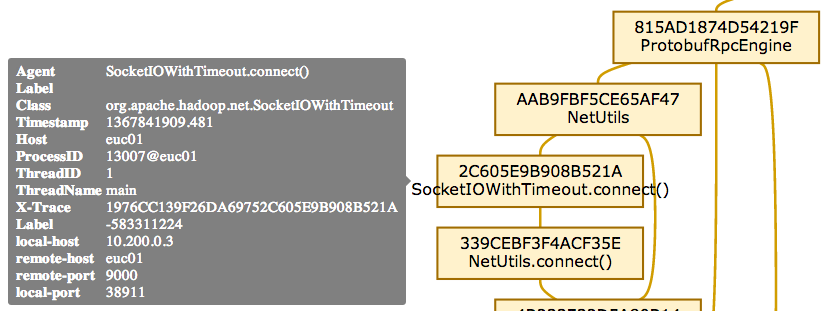
\includegraphics[width=0.7\textwidth]{figures/xtrace-example2.png}
\caption{An snippet of X-Trace events logged during a Hadoop execution.}
\label{fig:xtrace}
\end{figure}

\subsection{Lower-level Tracing}
\label{ssec:low}
In order to capture low-level information about all TCP flows created by Hadoop 
we use the popular packet-header capturing mechanism \emph{tcpdump}~\cite{tcpdump}.
Upon executing a job in a cluster of machines we initiate tcpdump to capture the 
first 120 bytes of each packet, which for our purposes encompasses the entirety of 
the header of a TCP packet. 

By capturing packet-header data we are then able to use tools like tstat~\cite{tstat}
and tcptrace~\cite{tcptrace} on the resulting tcpdump data. These tools allow us to 
easily retrieve statistics about the flows seen throughout the cluster such as 
average RTT values, flow duration, timeouts, fast re-transmissions, etc. 

Since X-Trace gives us a mechanism to expose the 5-tuple for each flow created by 
Hadoop and tcpdump also exposes a 5-tuple for each packet we can easily correlate
the application events that create sockets to the tcpdump captured packets by 
pairing up 5-tuples. In our implementation after completing a set of jobs we 
shutdown tcpdump, collect all the resulting tcpdump data, Hadoop logs, etc. and 
post-process the data to create a general JSON structure. This JSON structure maps
a flow ID (essentially the 5-tuple) to various application and low-level details. 
This JSON structure is later used in Section~\ref{sec:viz} to aid in visualizing the 
progression of events in the cluster.

\subsection{Tracing Results}
\label{ssec:results}
%Non-dynamic results from tracing, e.g. tput graphs, sdn tests, etc.
%Figure~\ref{fig:avg_rtt_cdf}
Through the use of Hadoop capacity scheduler we are able to run multiple job's 
simultaneously. The following experiments used two unique sets of 15GB of 
random data generated through Hadoop's random writer job. The experiments themselves
consisted of two simultaneous sort jobs on each newly generated data-set. Figure~\ref{fig:tput} 
shows all TCP flows created during the execution of the two sort jobs. Each line (or dot in 
many cases) represents the lifetime of a flow and its average throughput. Average throughput 
of a given flow is a function of total bytes transferred and the flow's total duration time.
This represents a basic indicator of the flow's throughput but does not take into account 
when the actual bytes where transferred, which means that traffic that is bursty is not
represented.

In addition to low-level TCP flow throughput information Figure~\ref{fig:tput} also shows 
application-level information regarding what type of service the flow is associated with. 
Hadoop has several services and stages during its execution, which are decoded in the 
color-category table shown in Figure~\ref{fig:cats}. 

Figure~\ref{fig:duration_cdf}

\begin{comment}
\begin{figure}
\centering
\begin{minipage}{.5\textwidth}
  \centering
  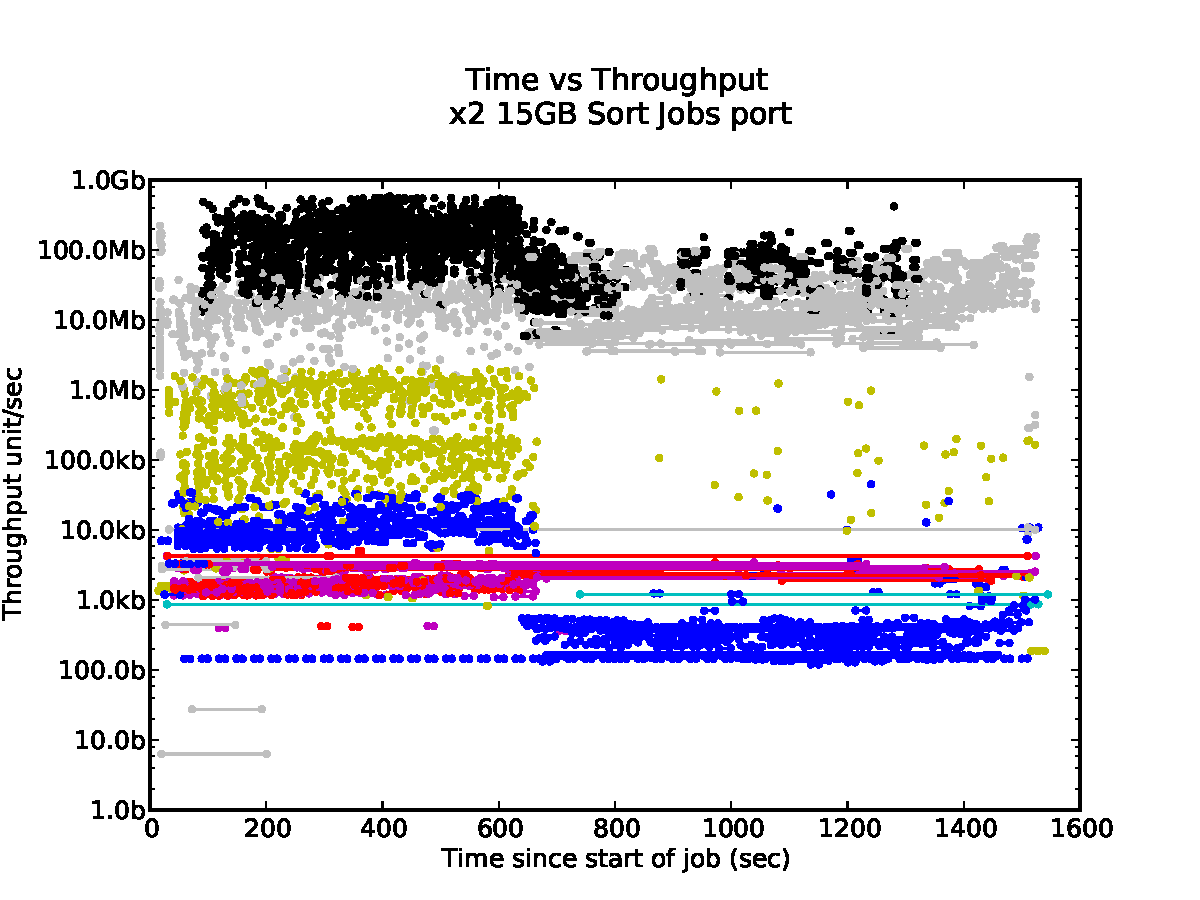
\includegraphics[width=.9\linewidth]{figures/clock_v_throughput_port.pdf}}
  \captionof{figure}{Average throughput of all Hadoop related flows over time.}
  \label{fig:tput}
\end{minipage}%
\begin{minipage}{.5\textwidth}
  \centering
  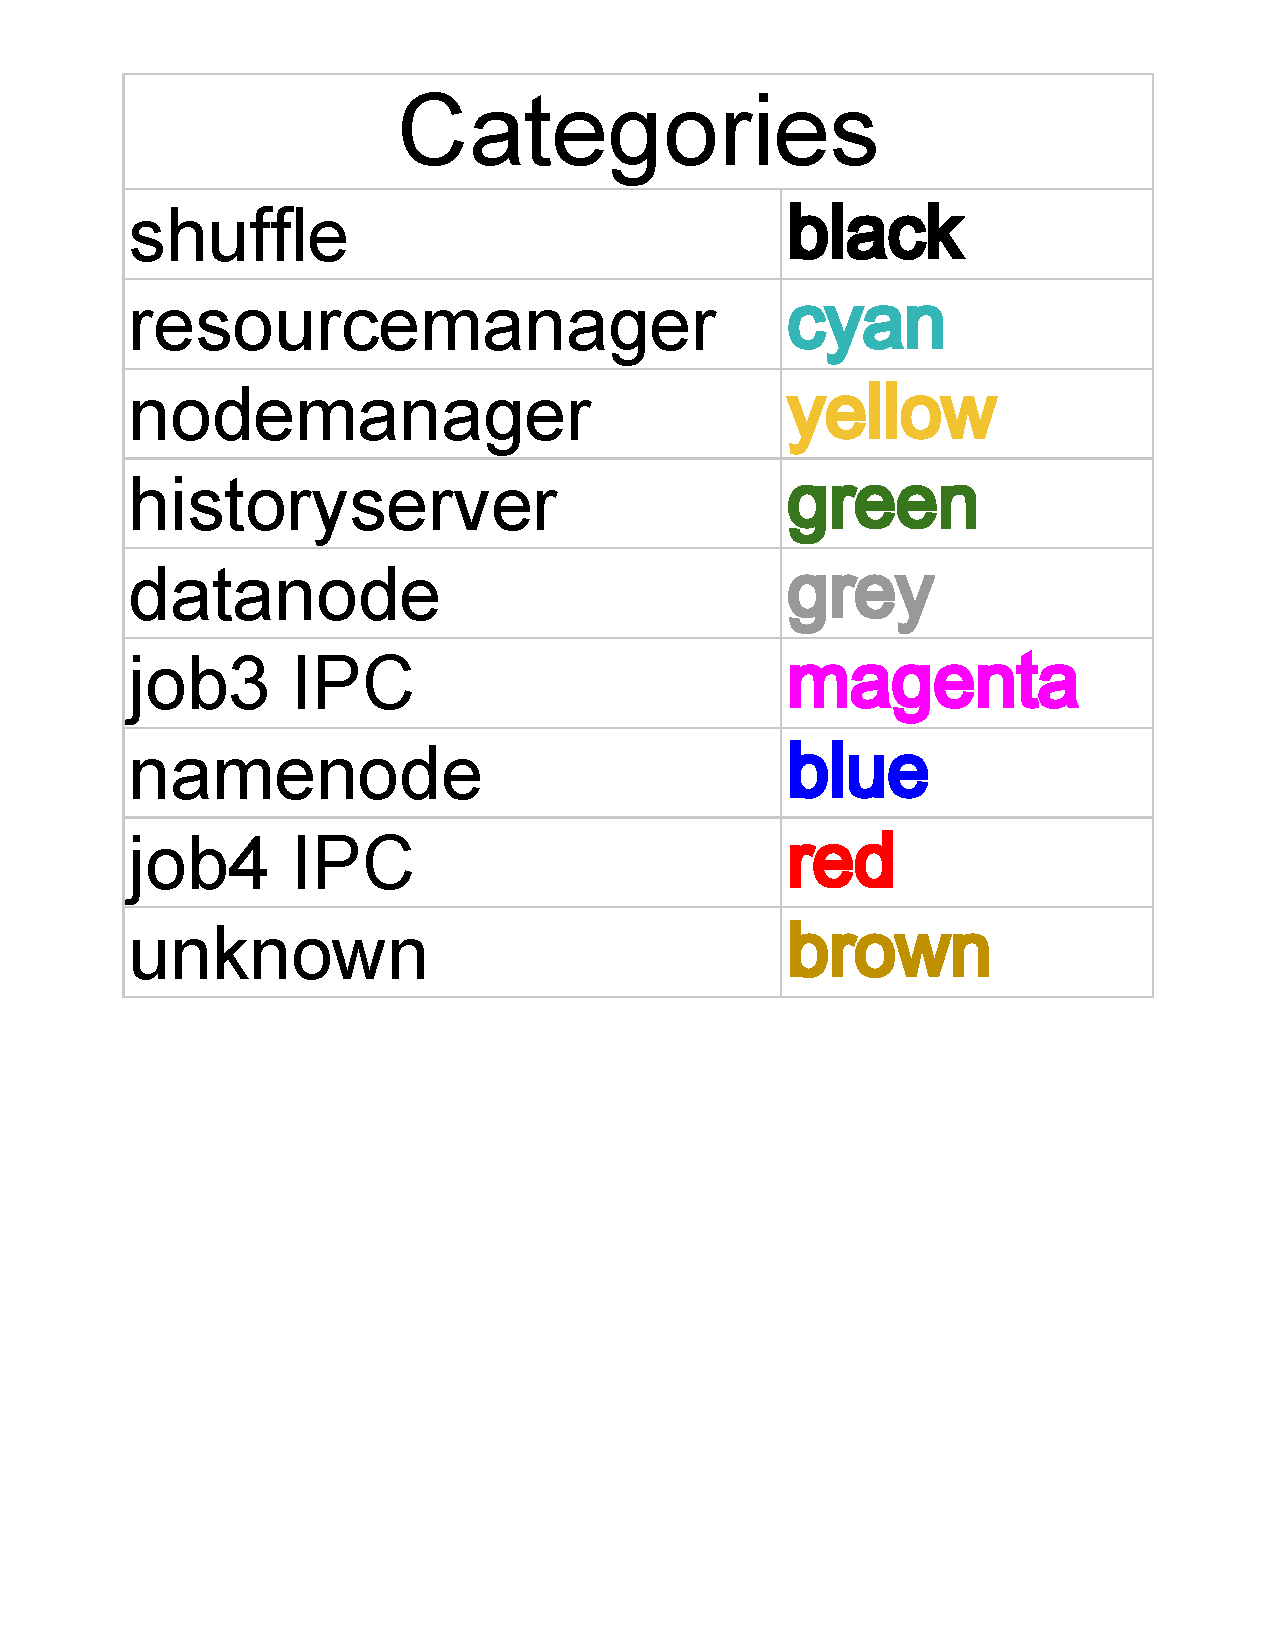
\includegraphics[width=.9\linewidth]{figures/categories.pdf}
  \captionof{figure}{Average RTTs for NameNode related flows.}
  \label{fig:foo}
\end{minipage}
\end{figure}
\end{comment}

\begin{figure}
\centering
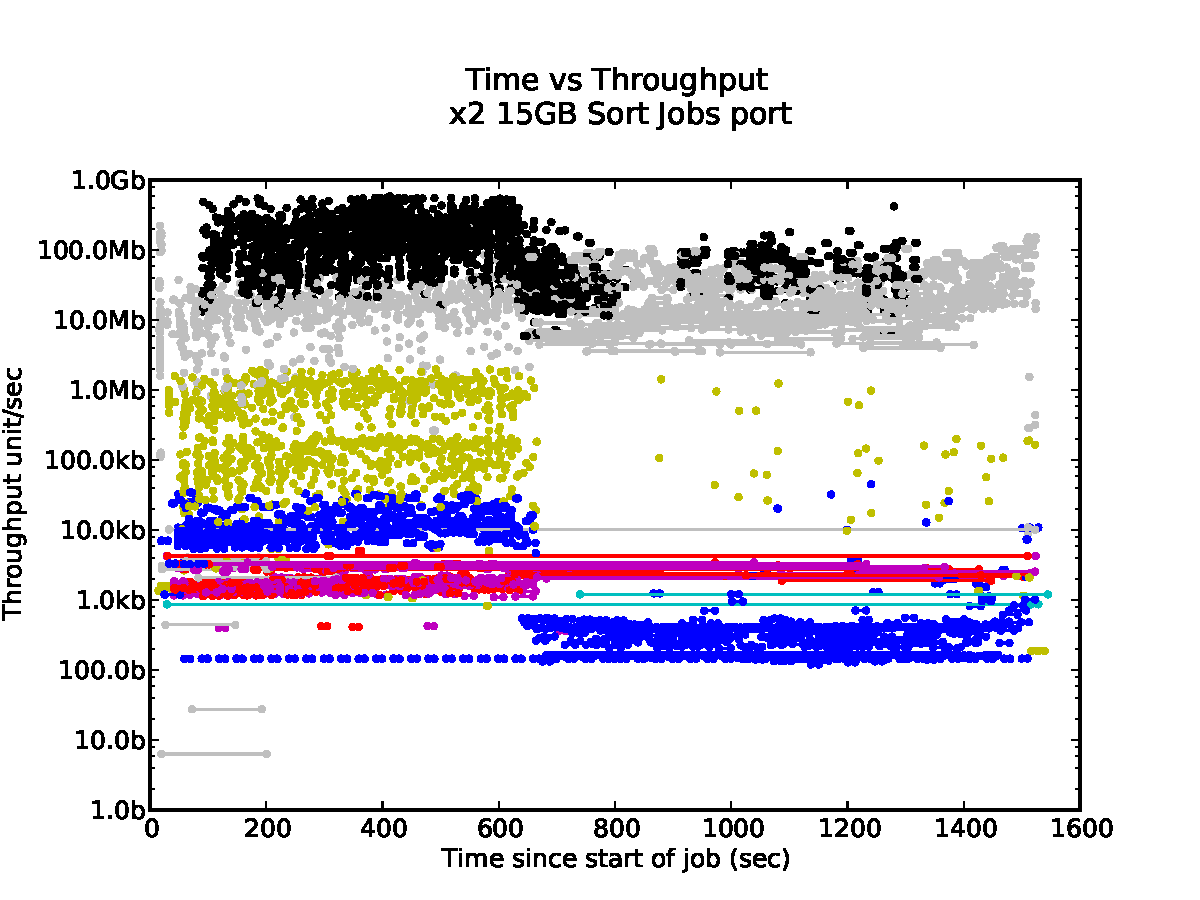
\includegraphics[width=0.7\textwidth]{figures/clock_v_throughput_port.pdf}
\caption{Average throughput of all Hadoop related flows over time.}
\label{fig:tput}
\end{figure}

\begin{figure}
\centering
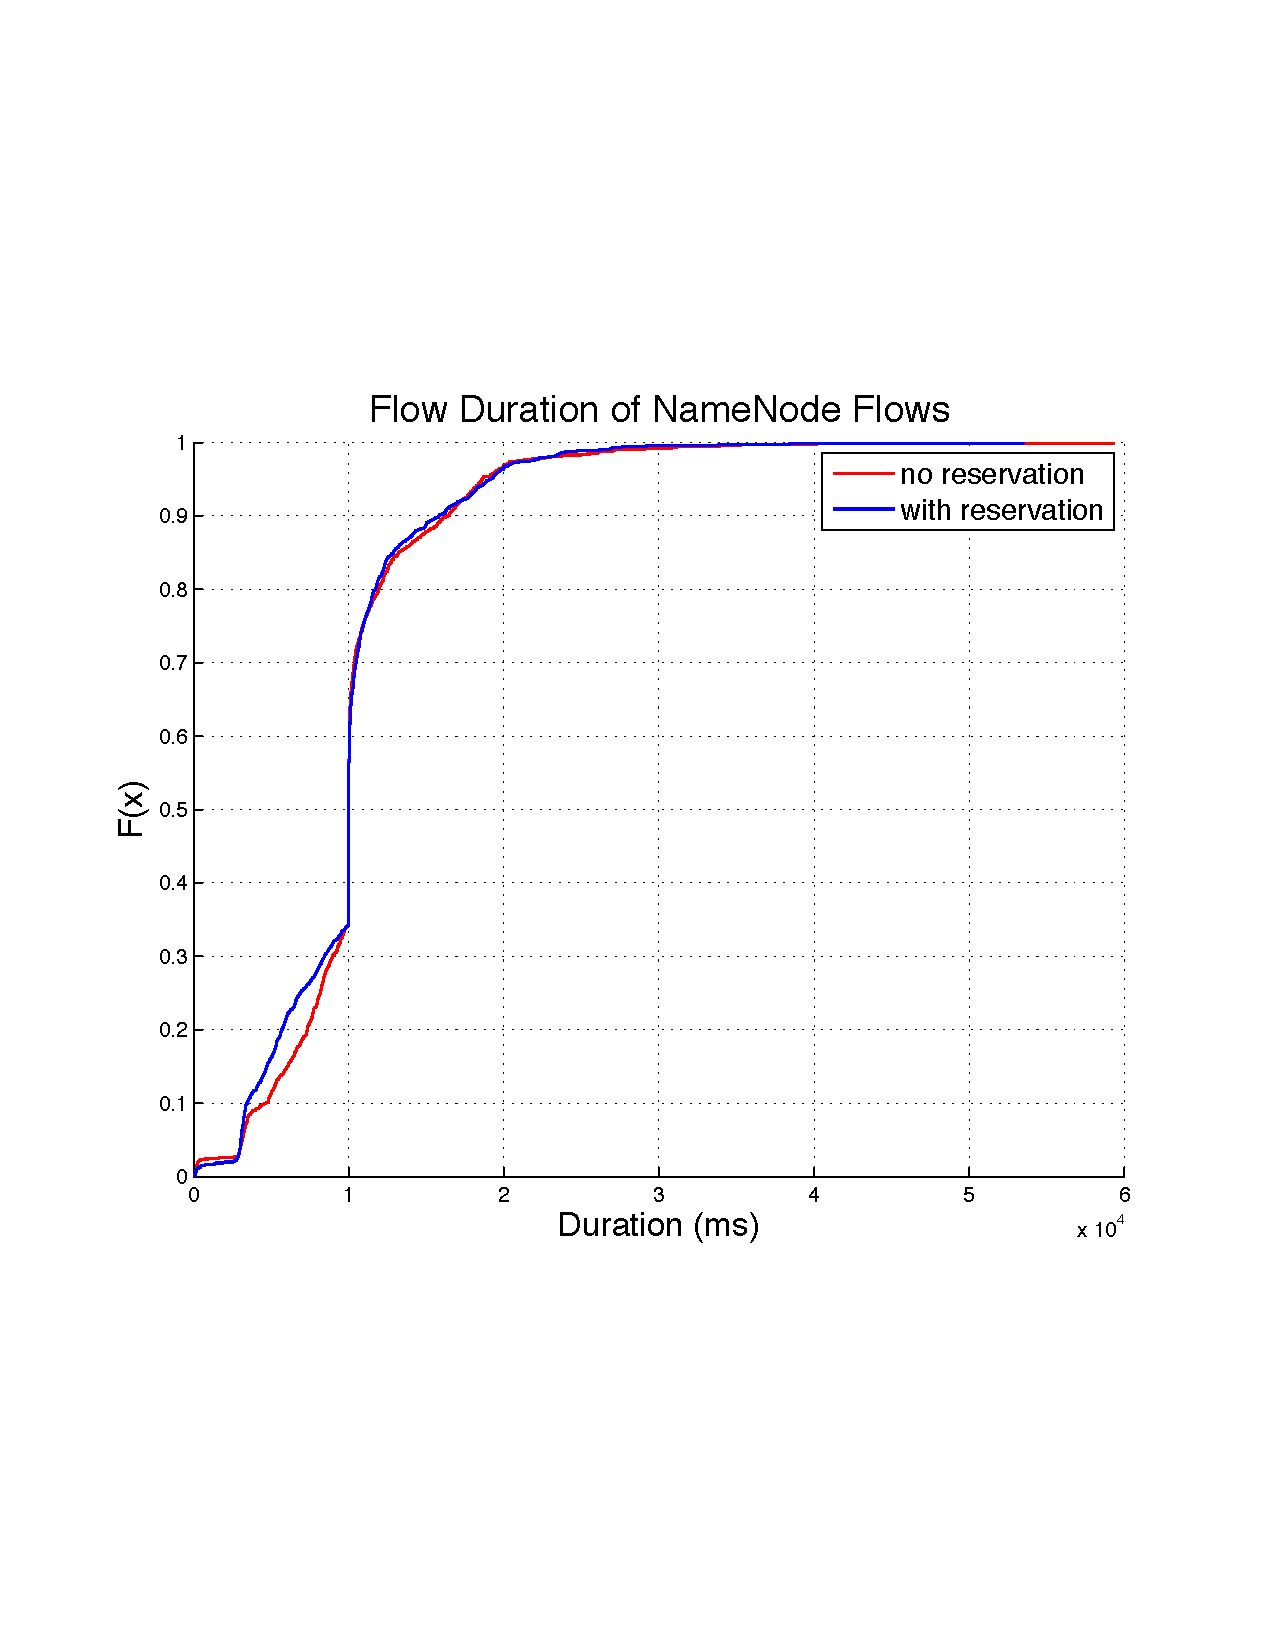
\includegraphics[width=0.7\textwidth]{figures/flow_durations.pdf}
\caption{Duration of NameNode related flows.}
\label{fig:duration_cdf}
\end{figure}

